\documentclass{article}
\usepackage[top=1cm]{geometry}
\usepackage{graphicx}
\usepackage{subfig}
\title{Report 1}

\begin{document}
\begin{figure}
\centering
\begin{tabular}{cc}
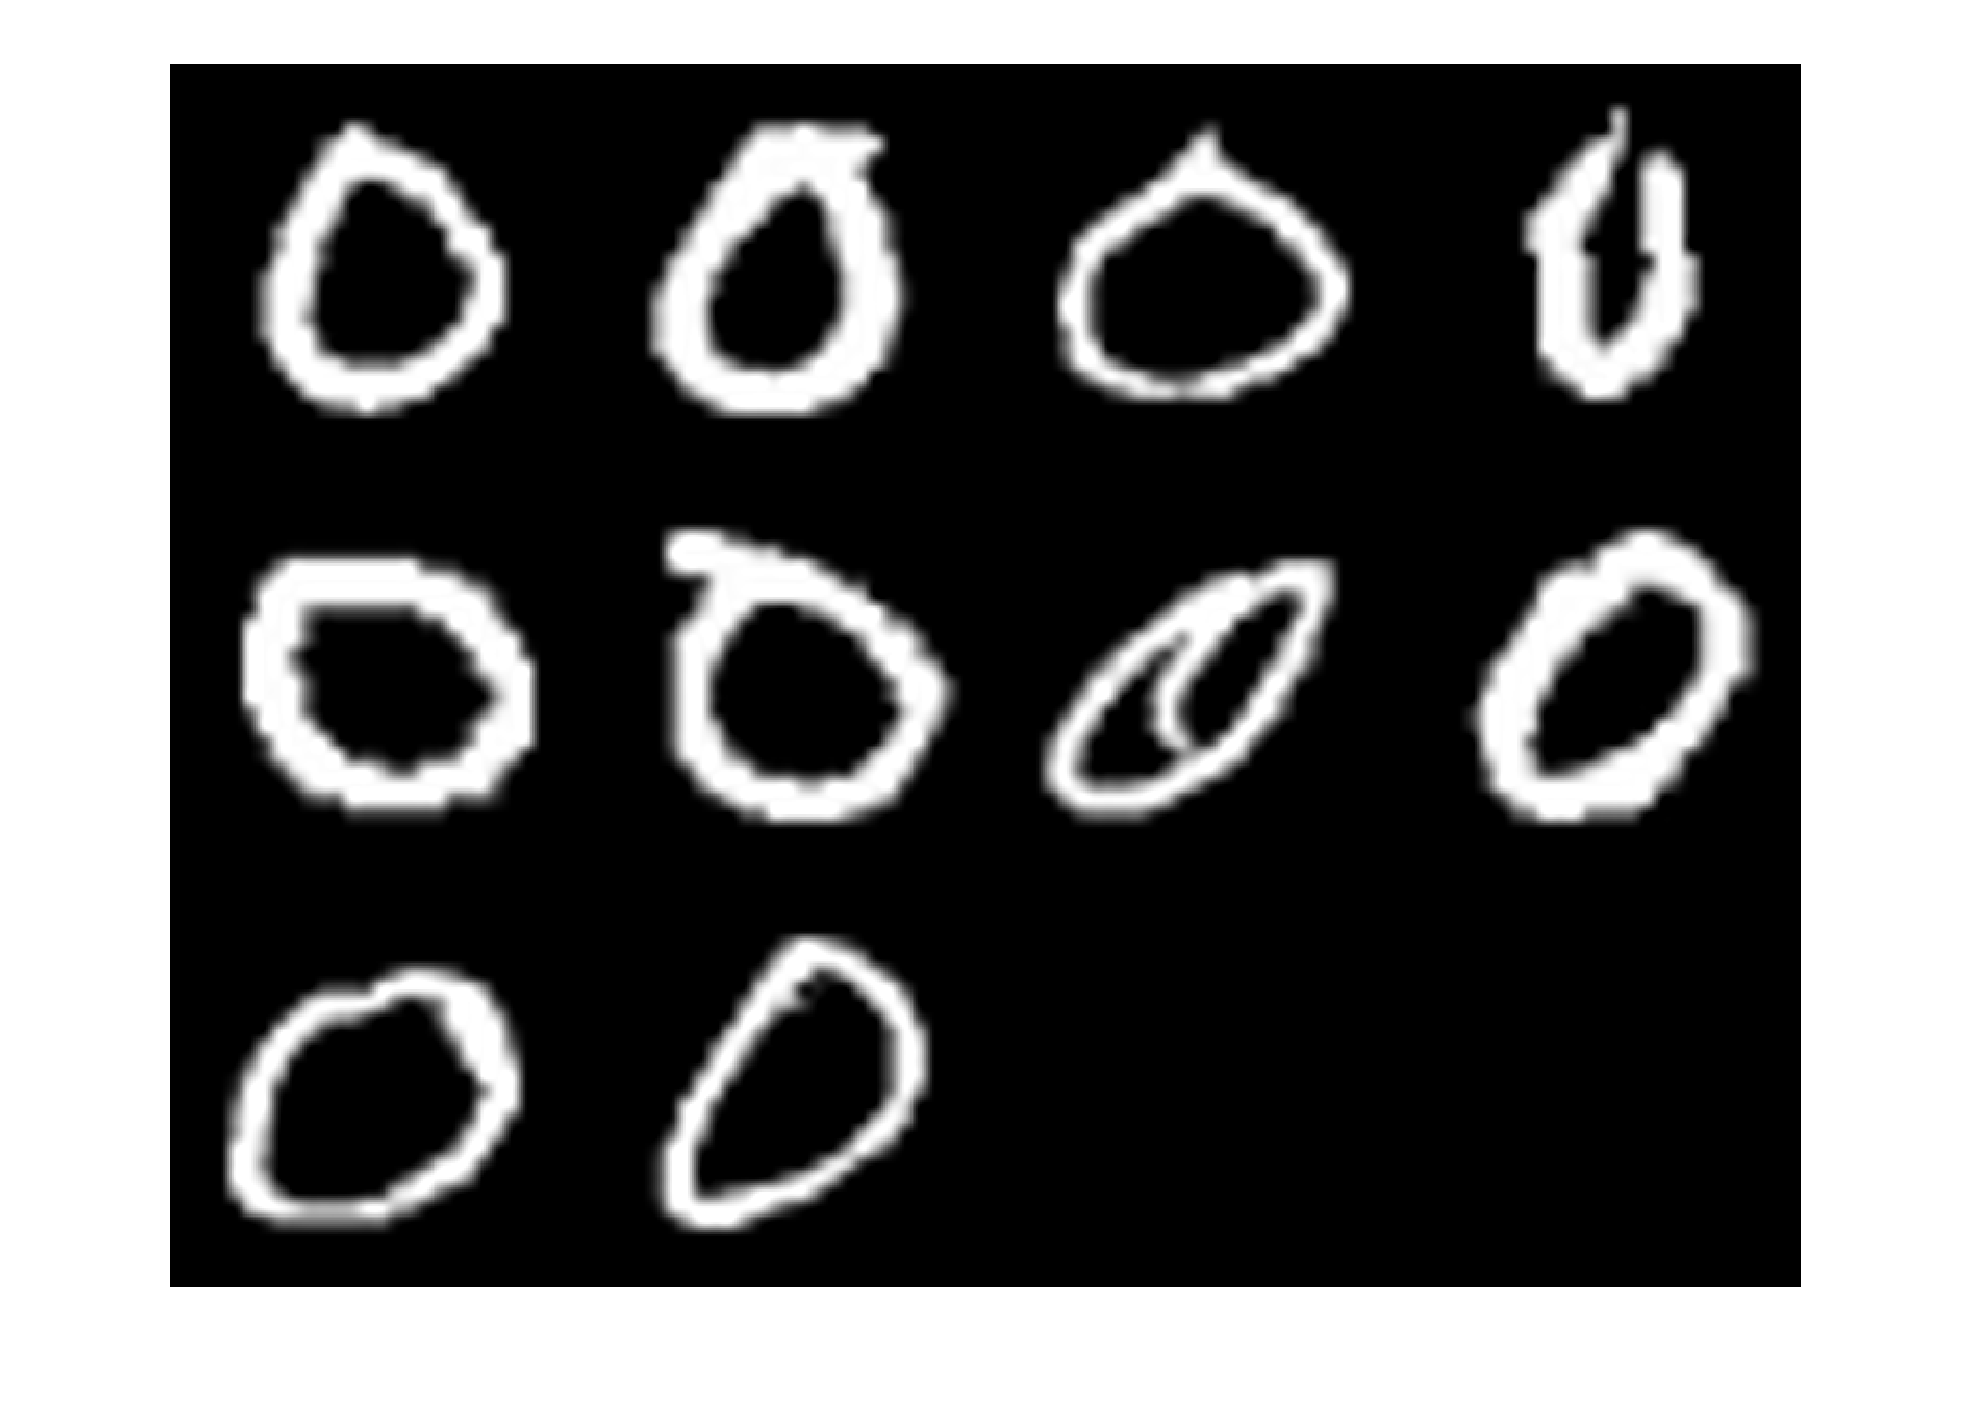
\includegraphics[width=55mm]{task1_1_imgs_class1.eps} &   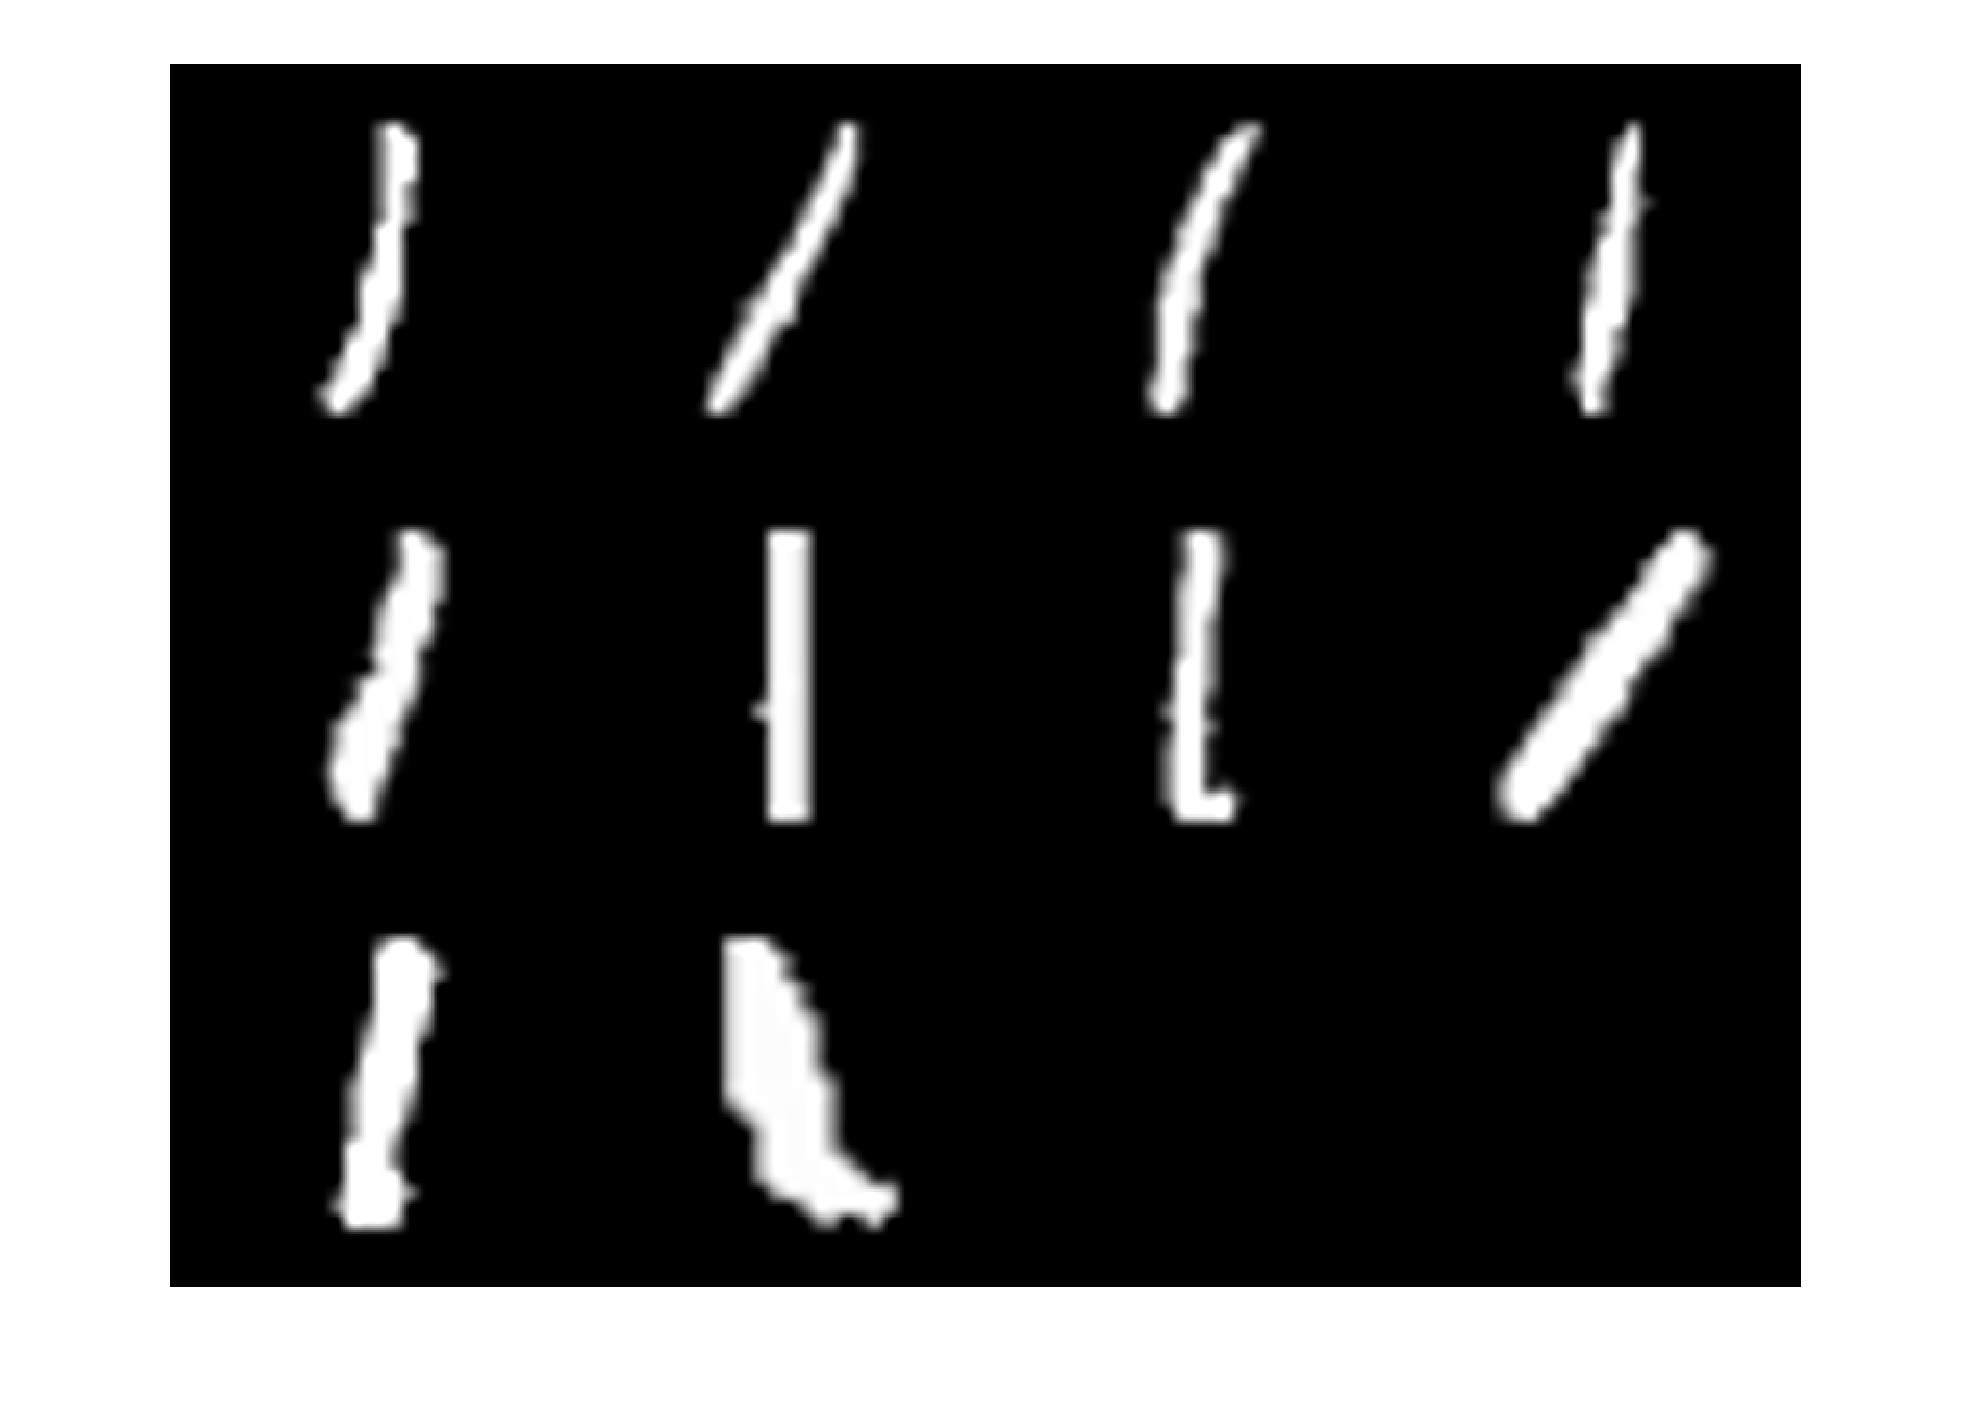
\includegraphics[width=55mm]{task1_1_imgs_class2.eps} \\
Class 1 & Class 2 \\[6pt]
 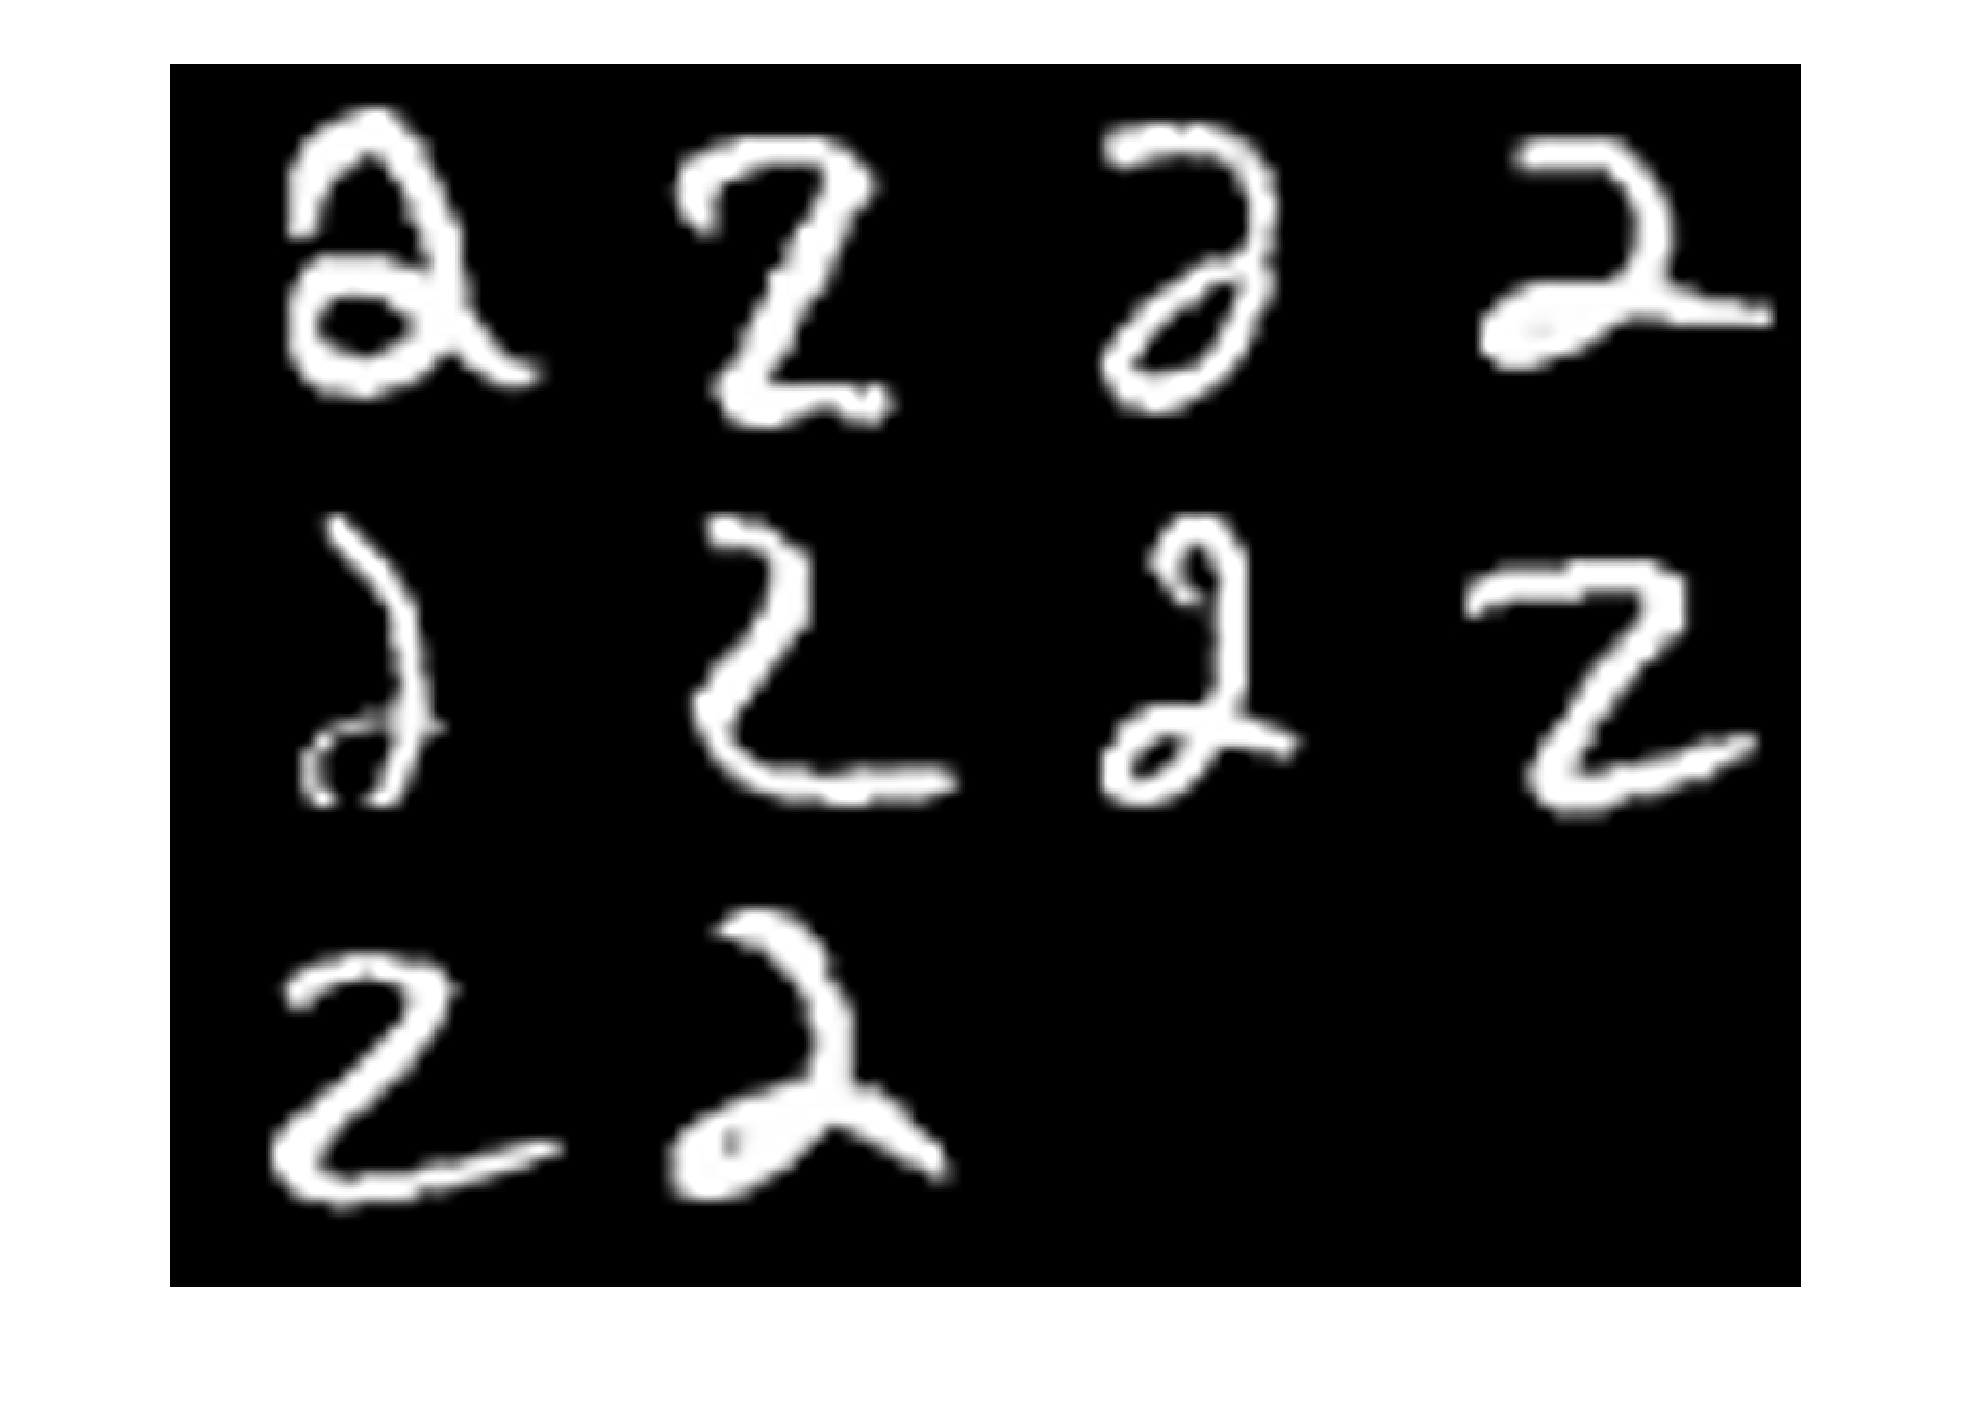
\includegraphics[width=55mm]{task1_1_imgs_class3.eps} &   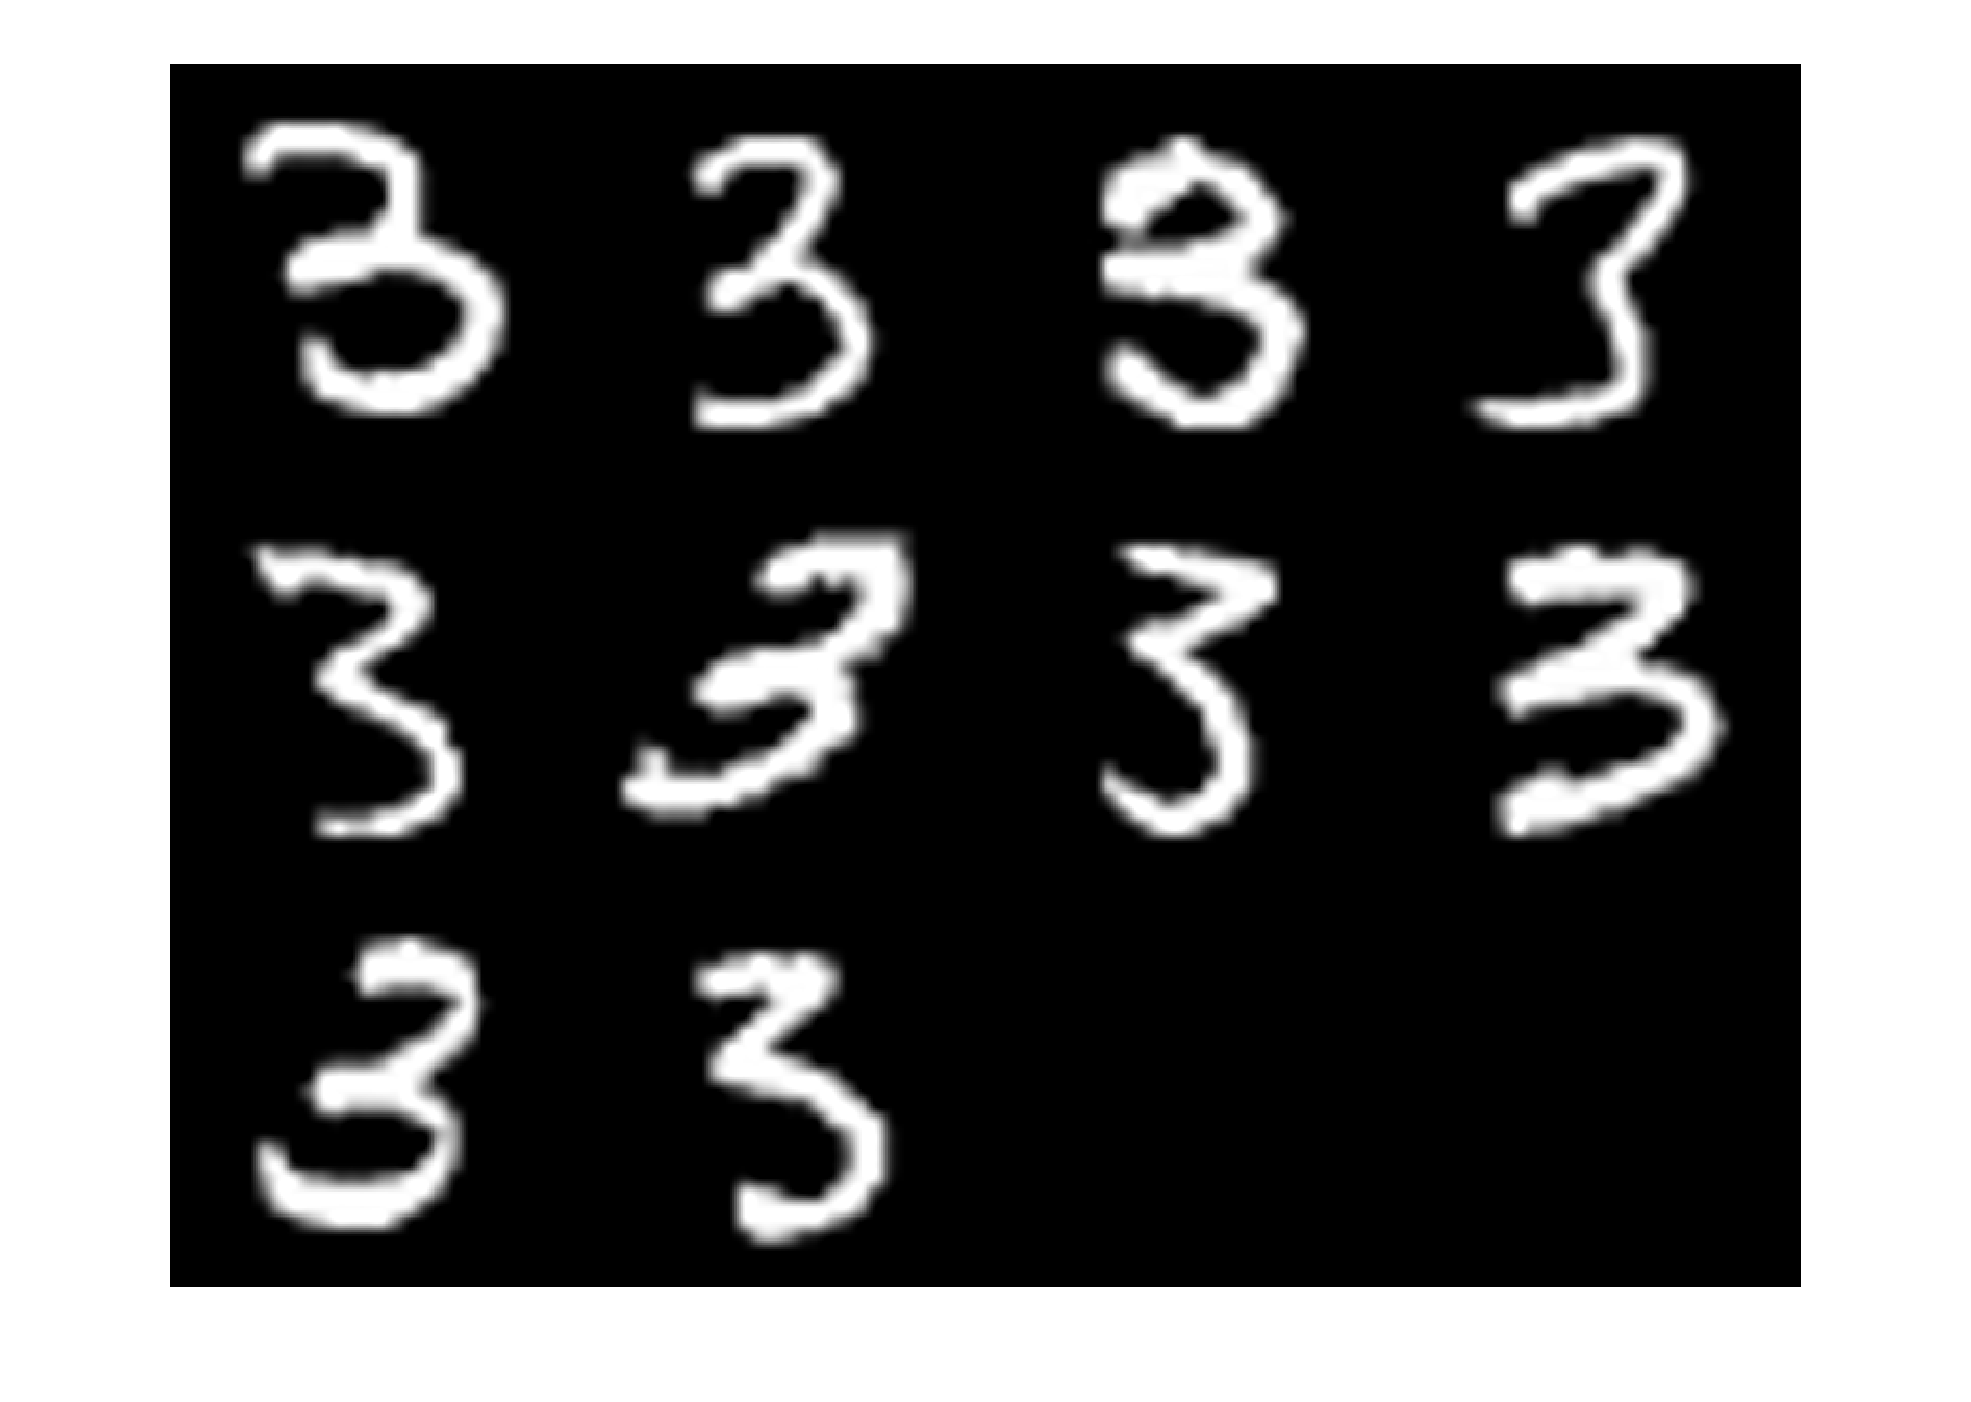
\includegraphics[width=55mm]{task1_1_imgs_class4.eps} \\
     Class 3 & Class 4 \\[6pt]
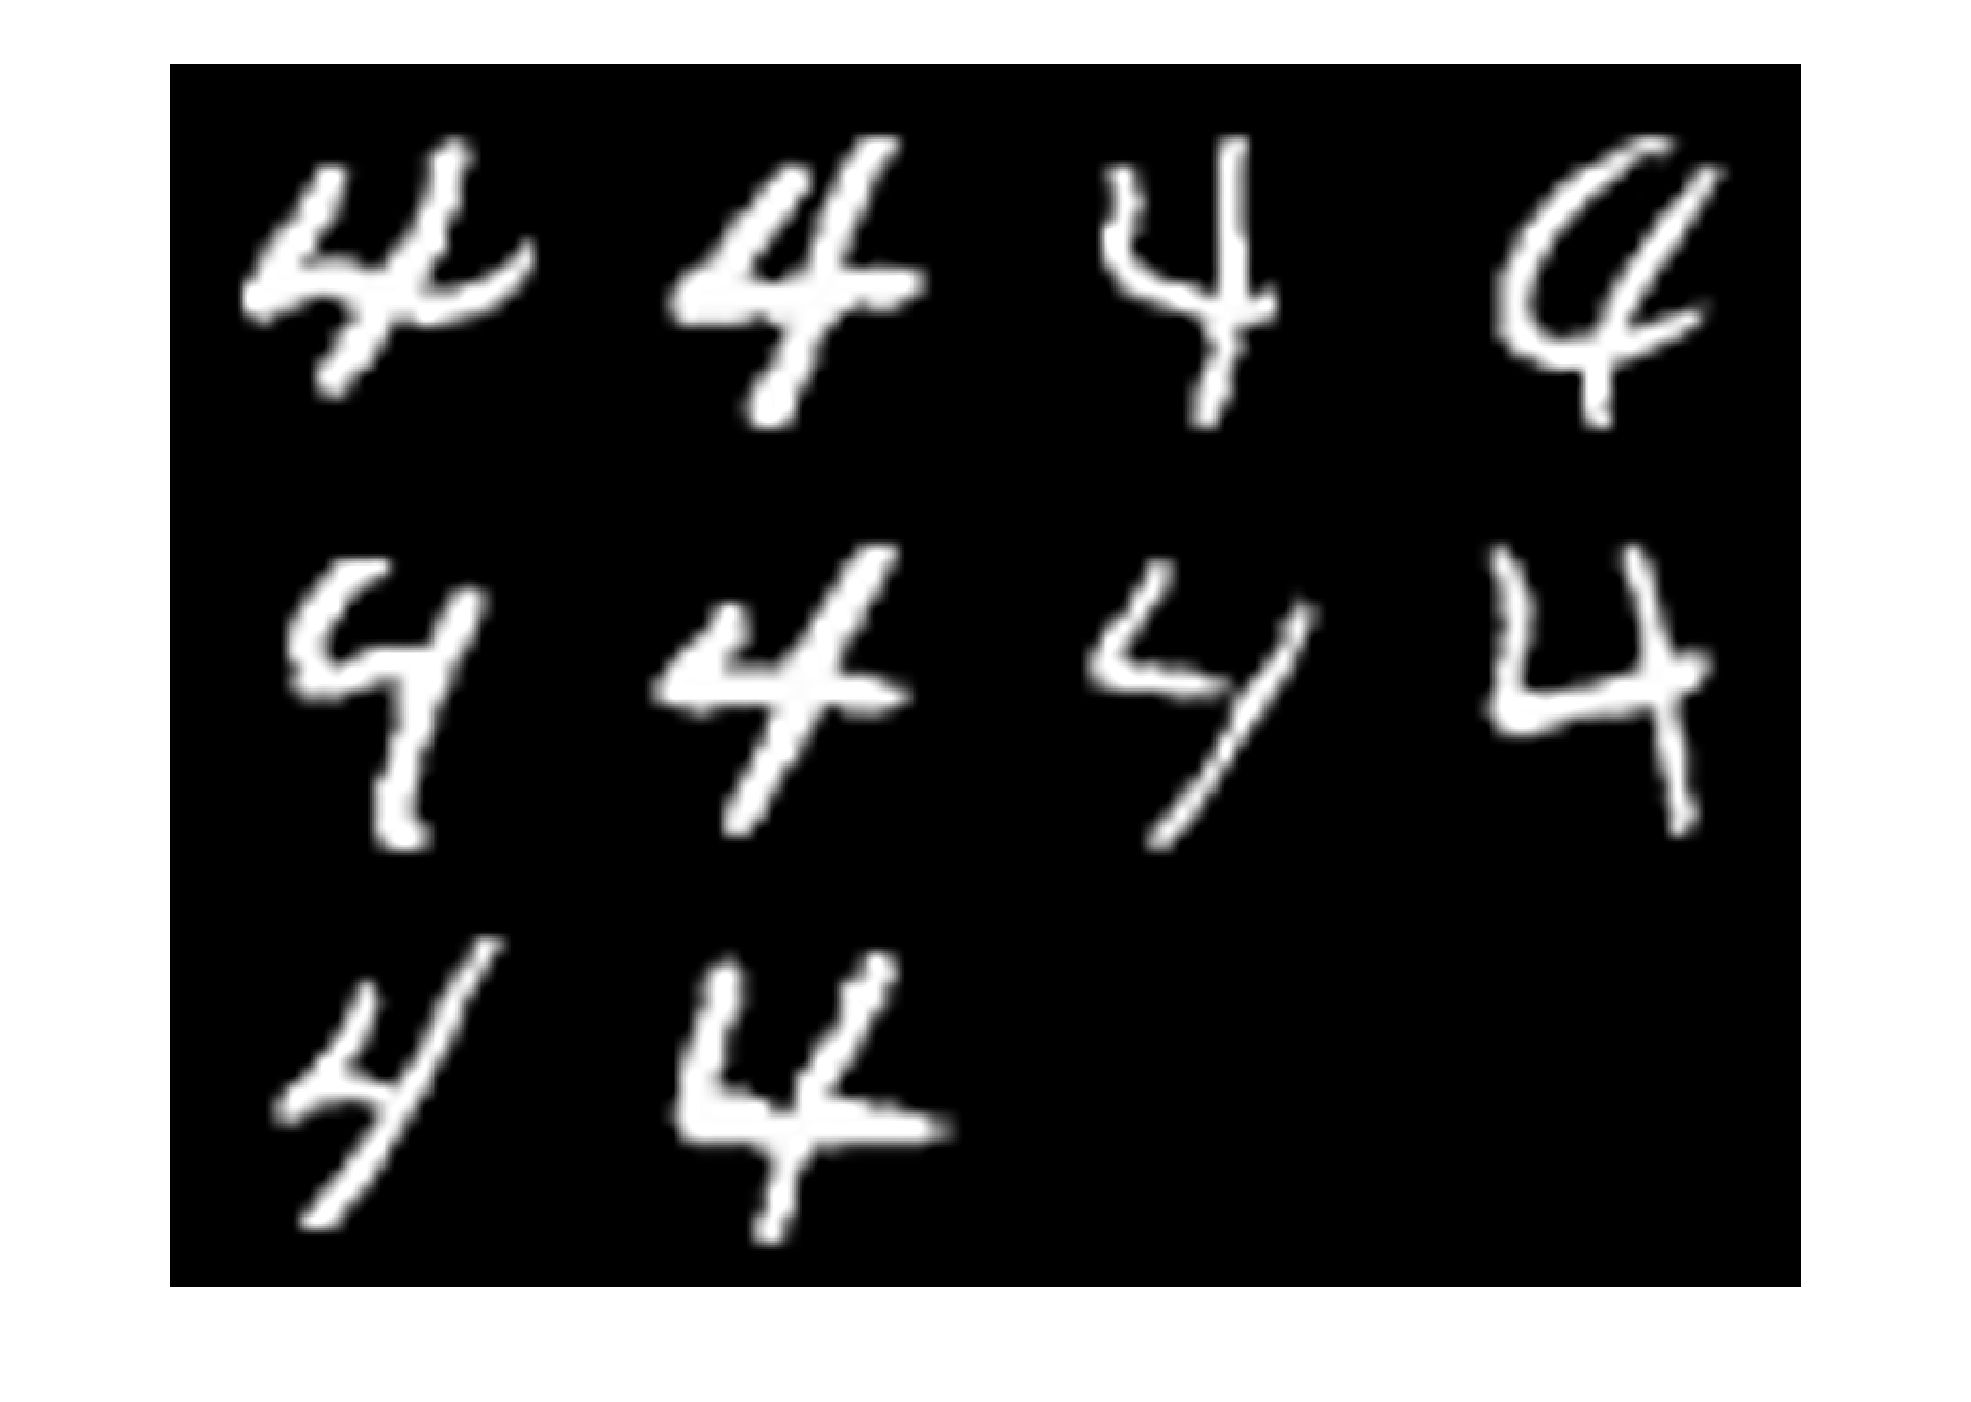
\includegraphics[width=55mm]{task1_1_imgs_class5.eps} &   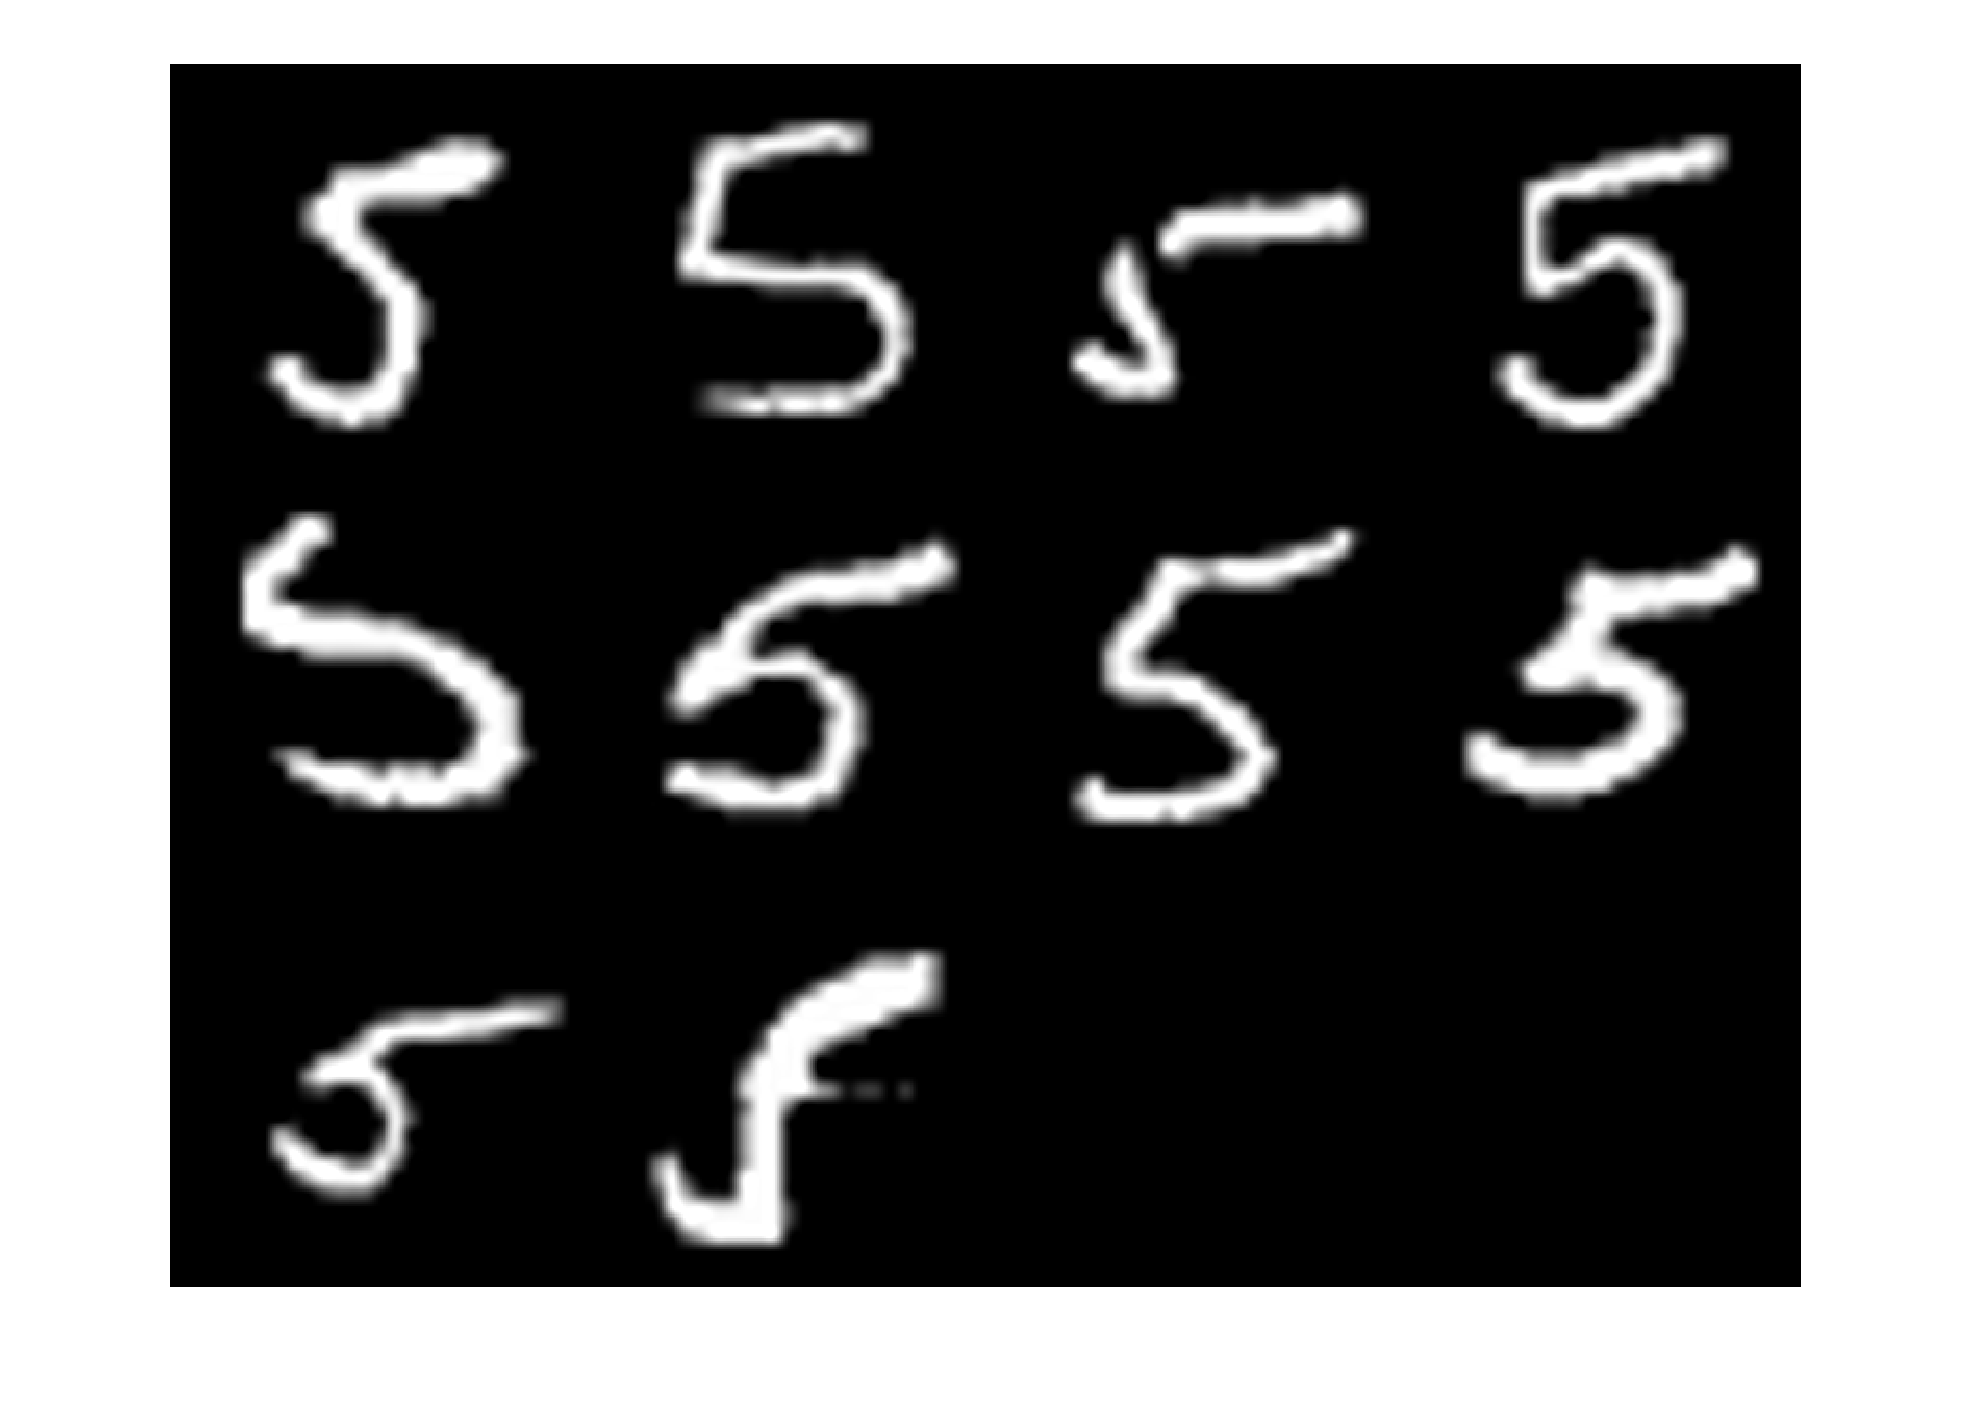
\includegraphics[width=55mm]{task1_1_imgs_class6.eps} \\
     Class 5 & Class 6 \\[6pt]
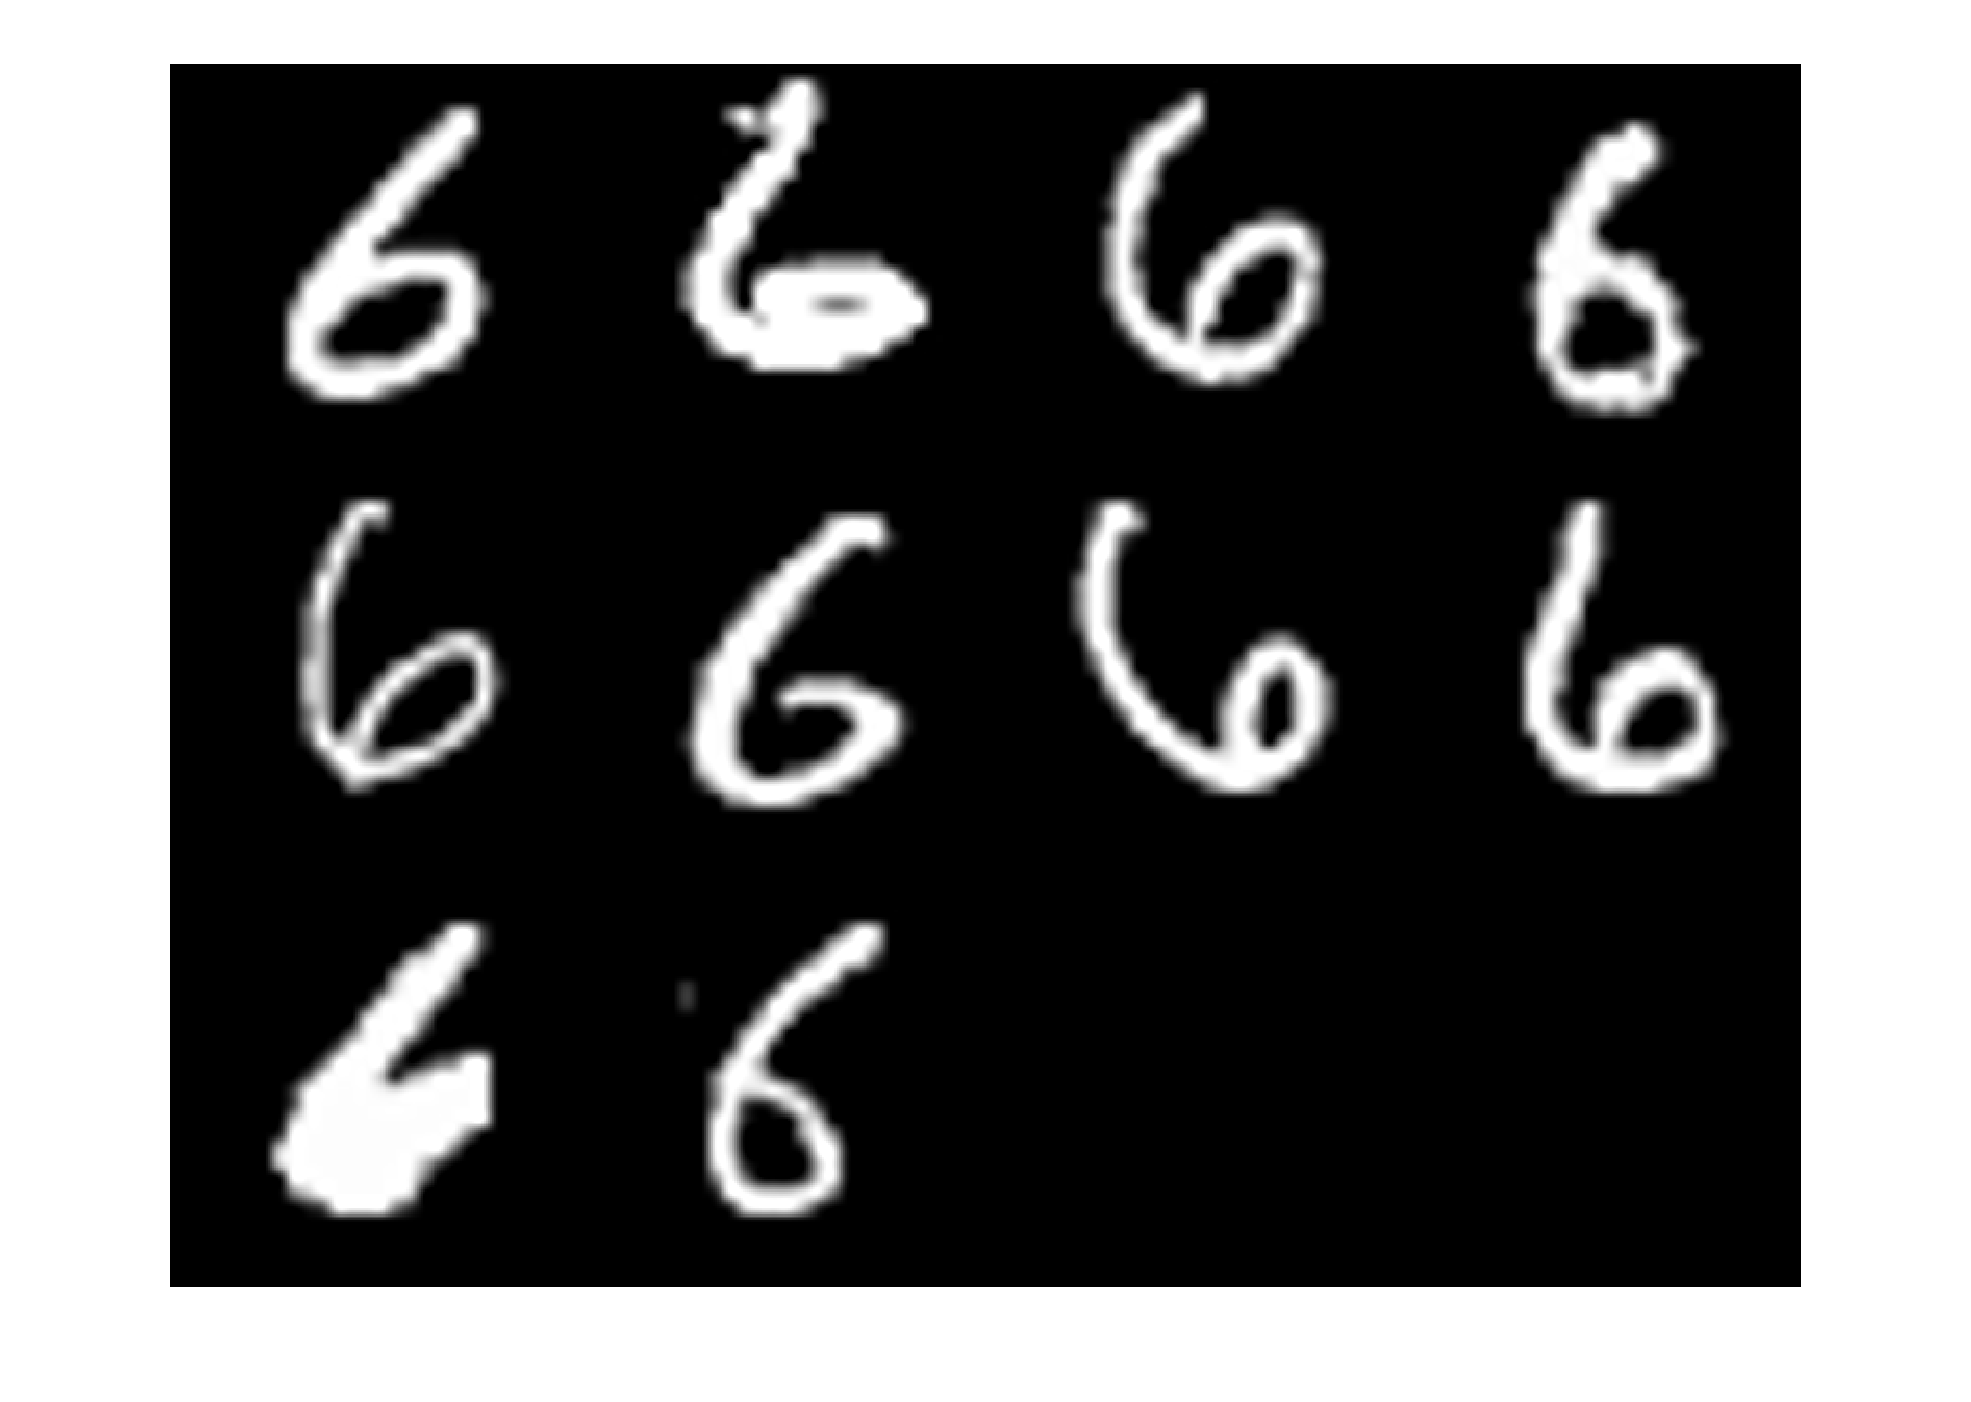
\includegraphics[width=55mm]{task1_1_imgs_class7.eps} &   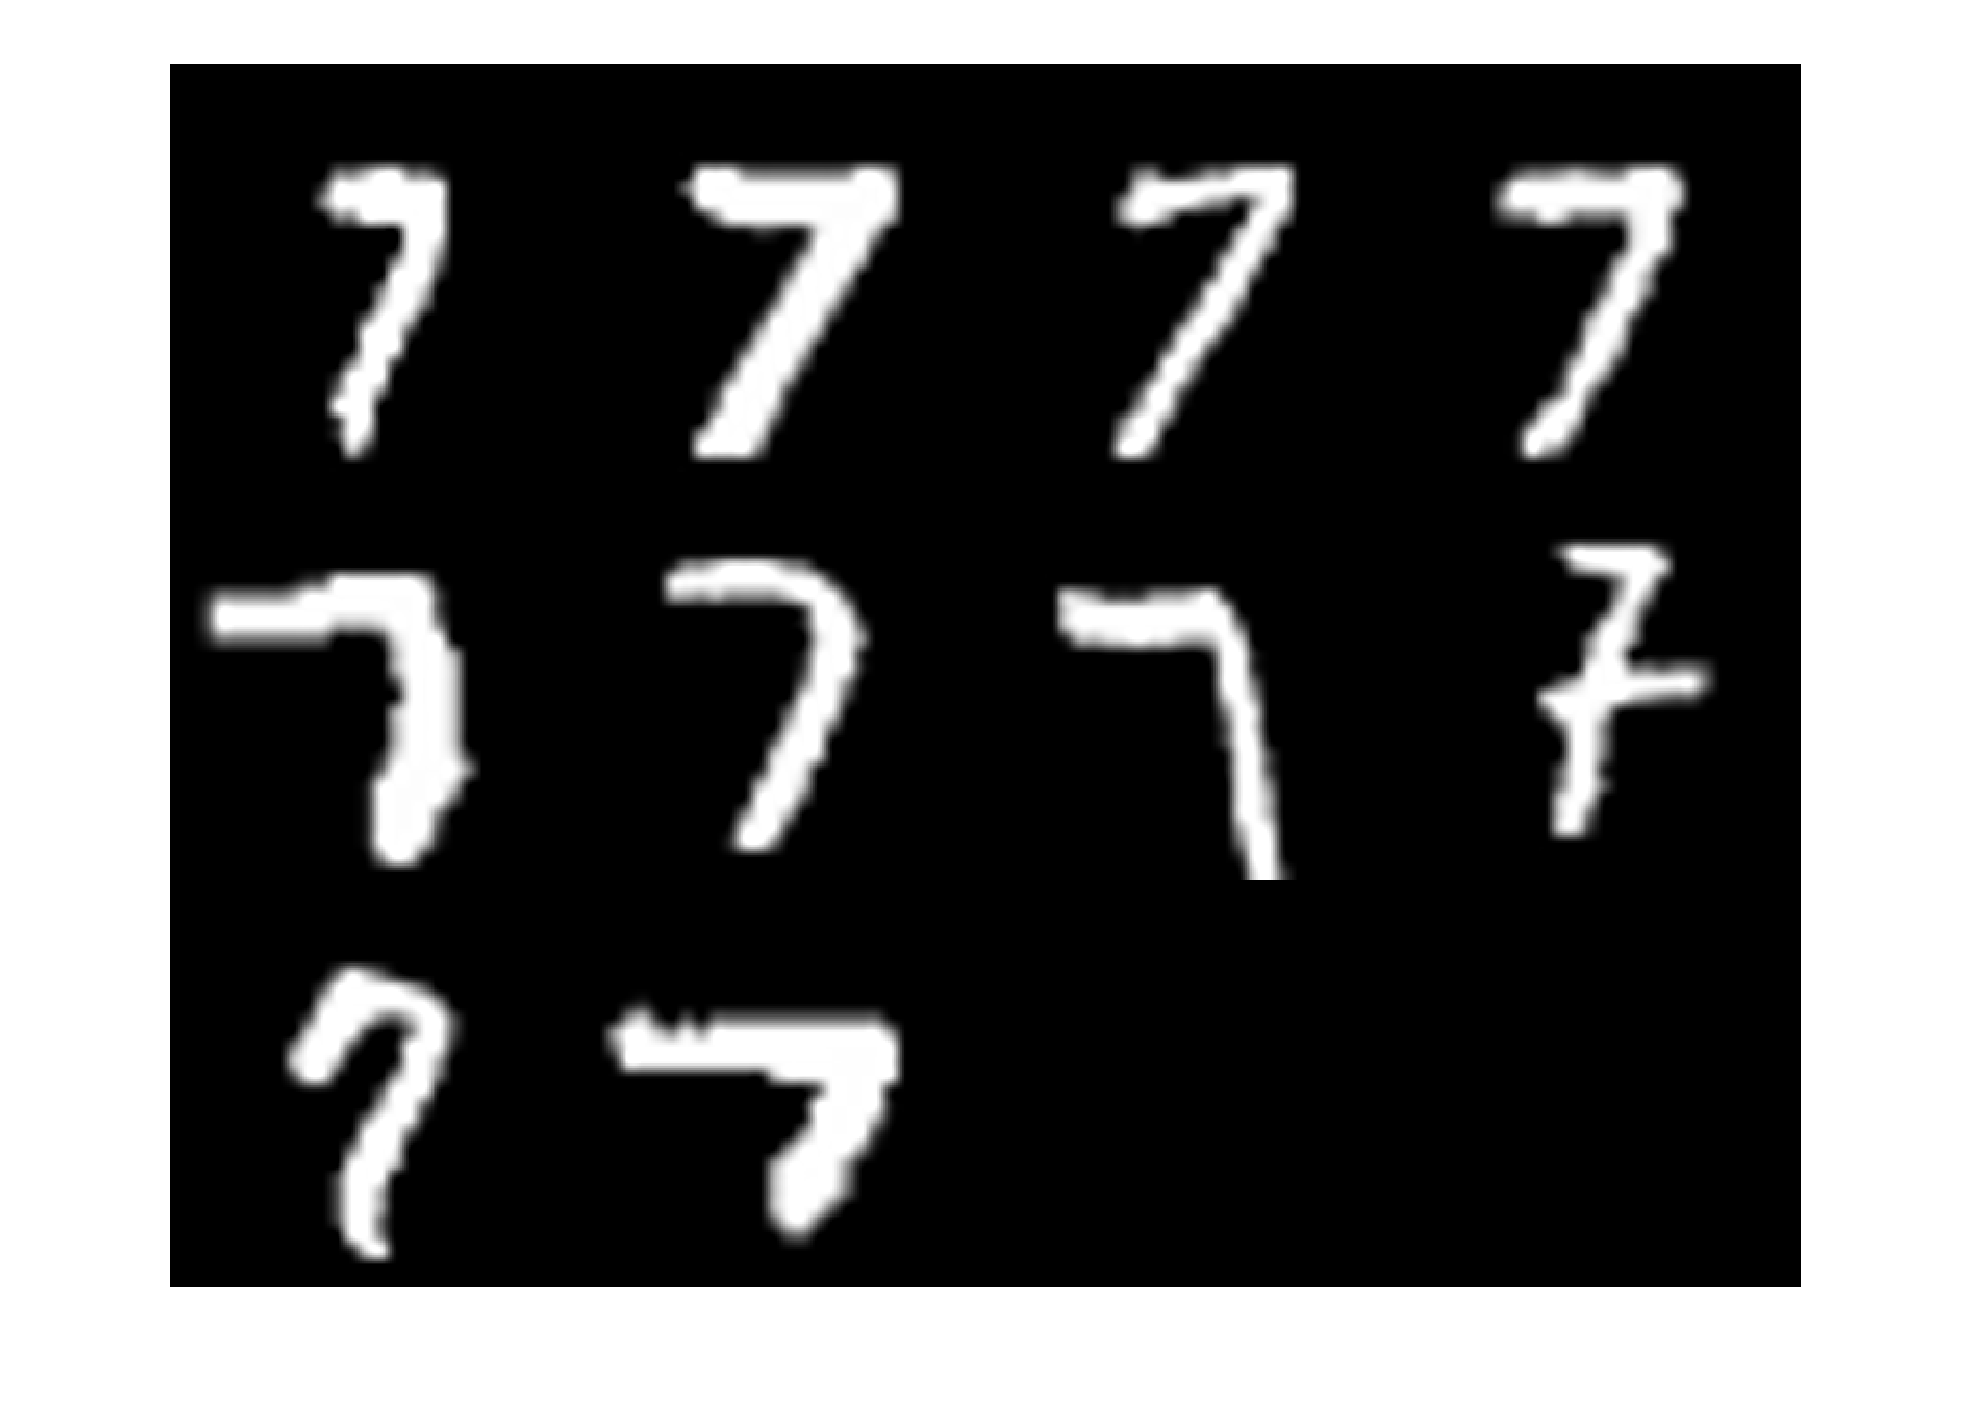
\includegraphics[width=55mm]{task1_1_imgs_class8.eps} \\
     Class 7 & Class 8 \\[6pt]
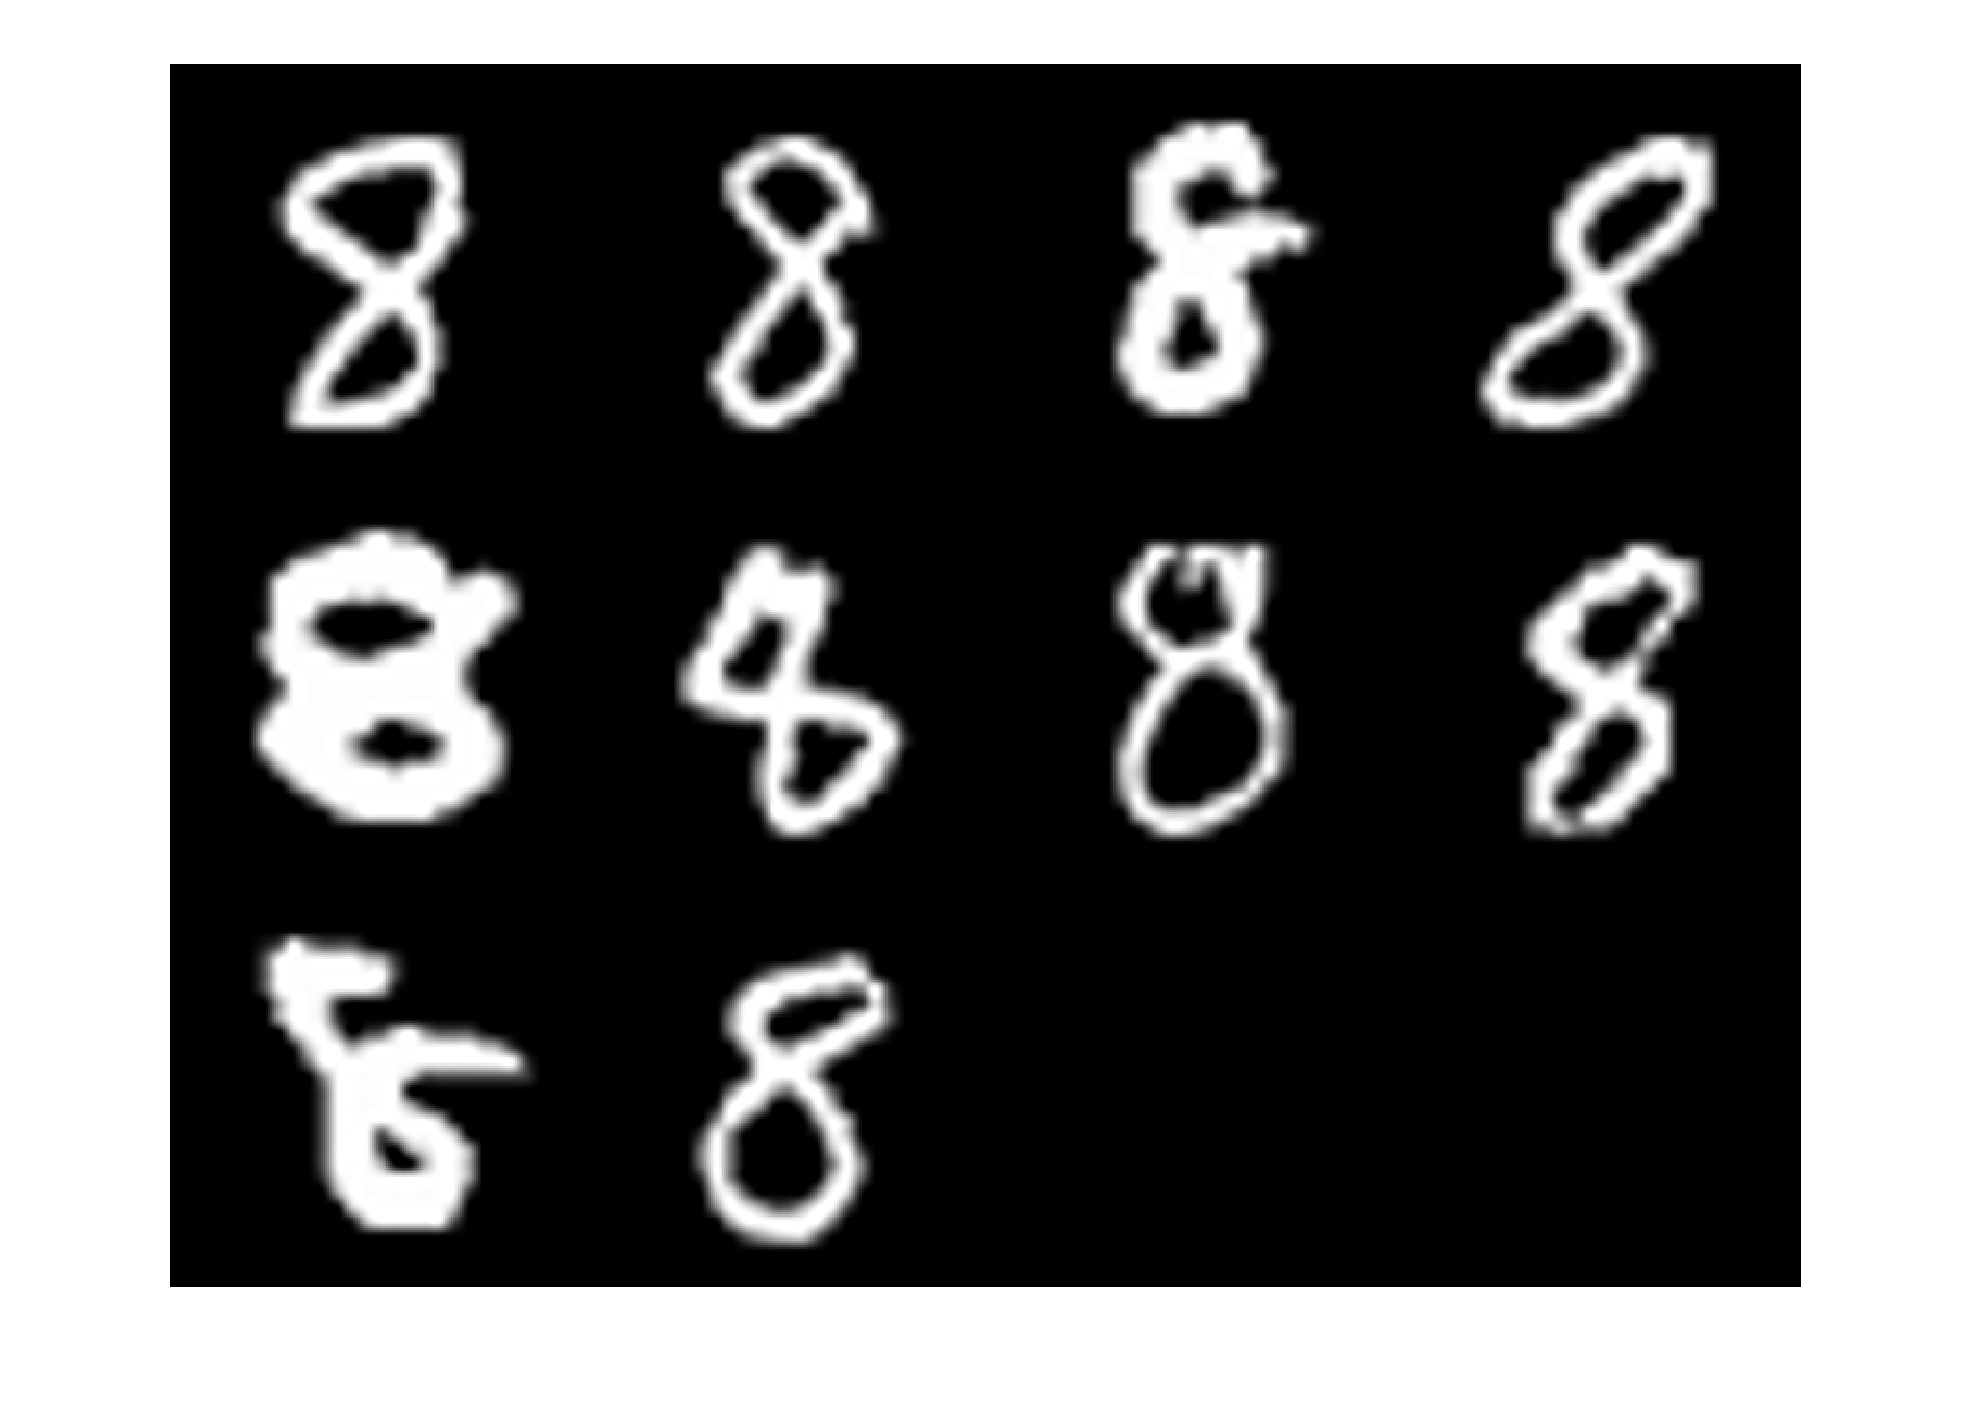
\includegraphics[width=55mm]{task1_1_imgs_class9.eps} &   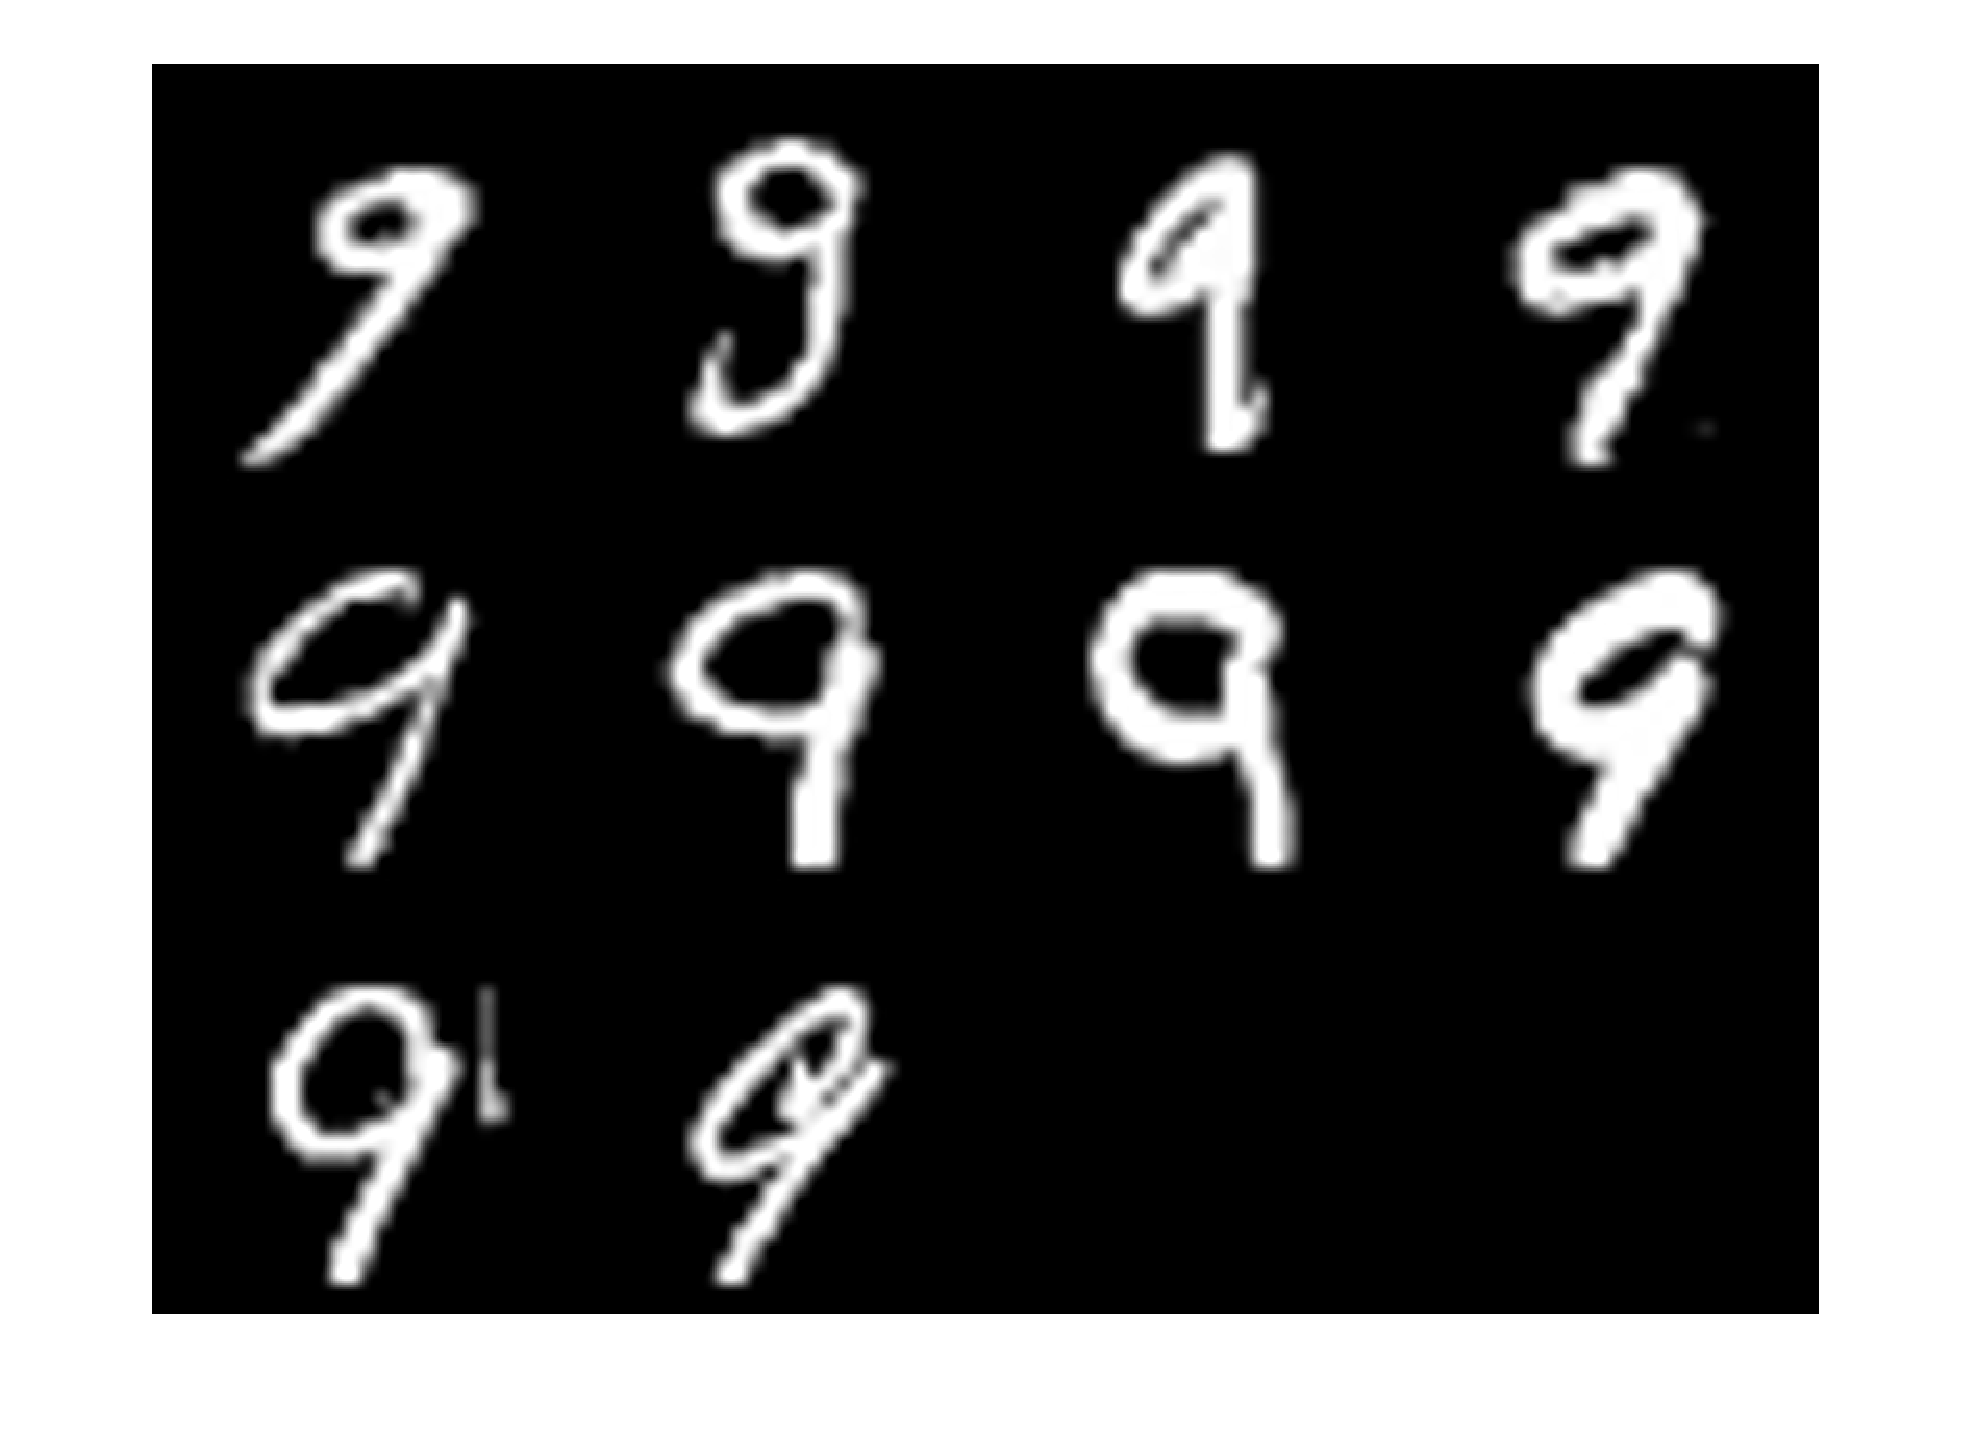
\includegraphics[width=55mm]{task1_1_imgs_class10.eps} \\
     Class 9 & Class 10 \\[6pt]
     
\end{tabular}
\caption{Task 1.1}
\end{figure}
\begin{figure}
 \centering
	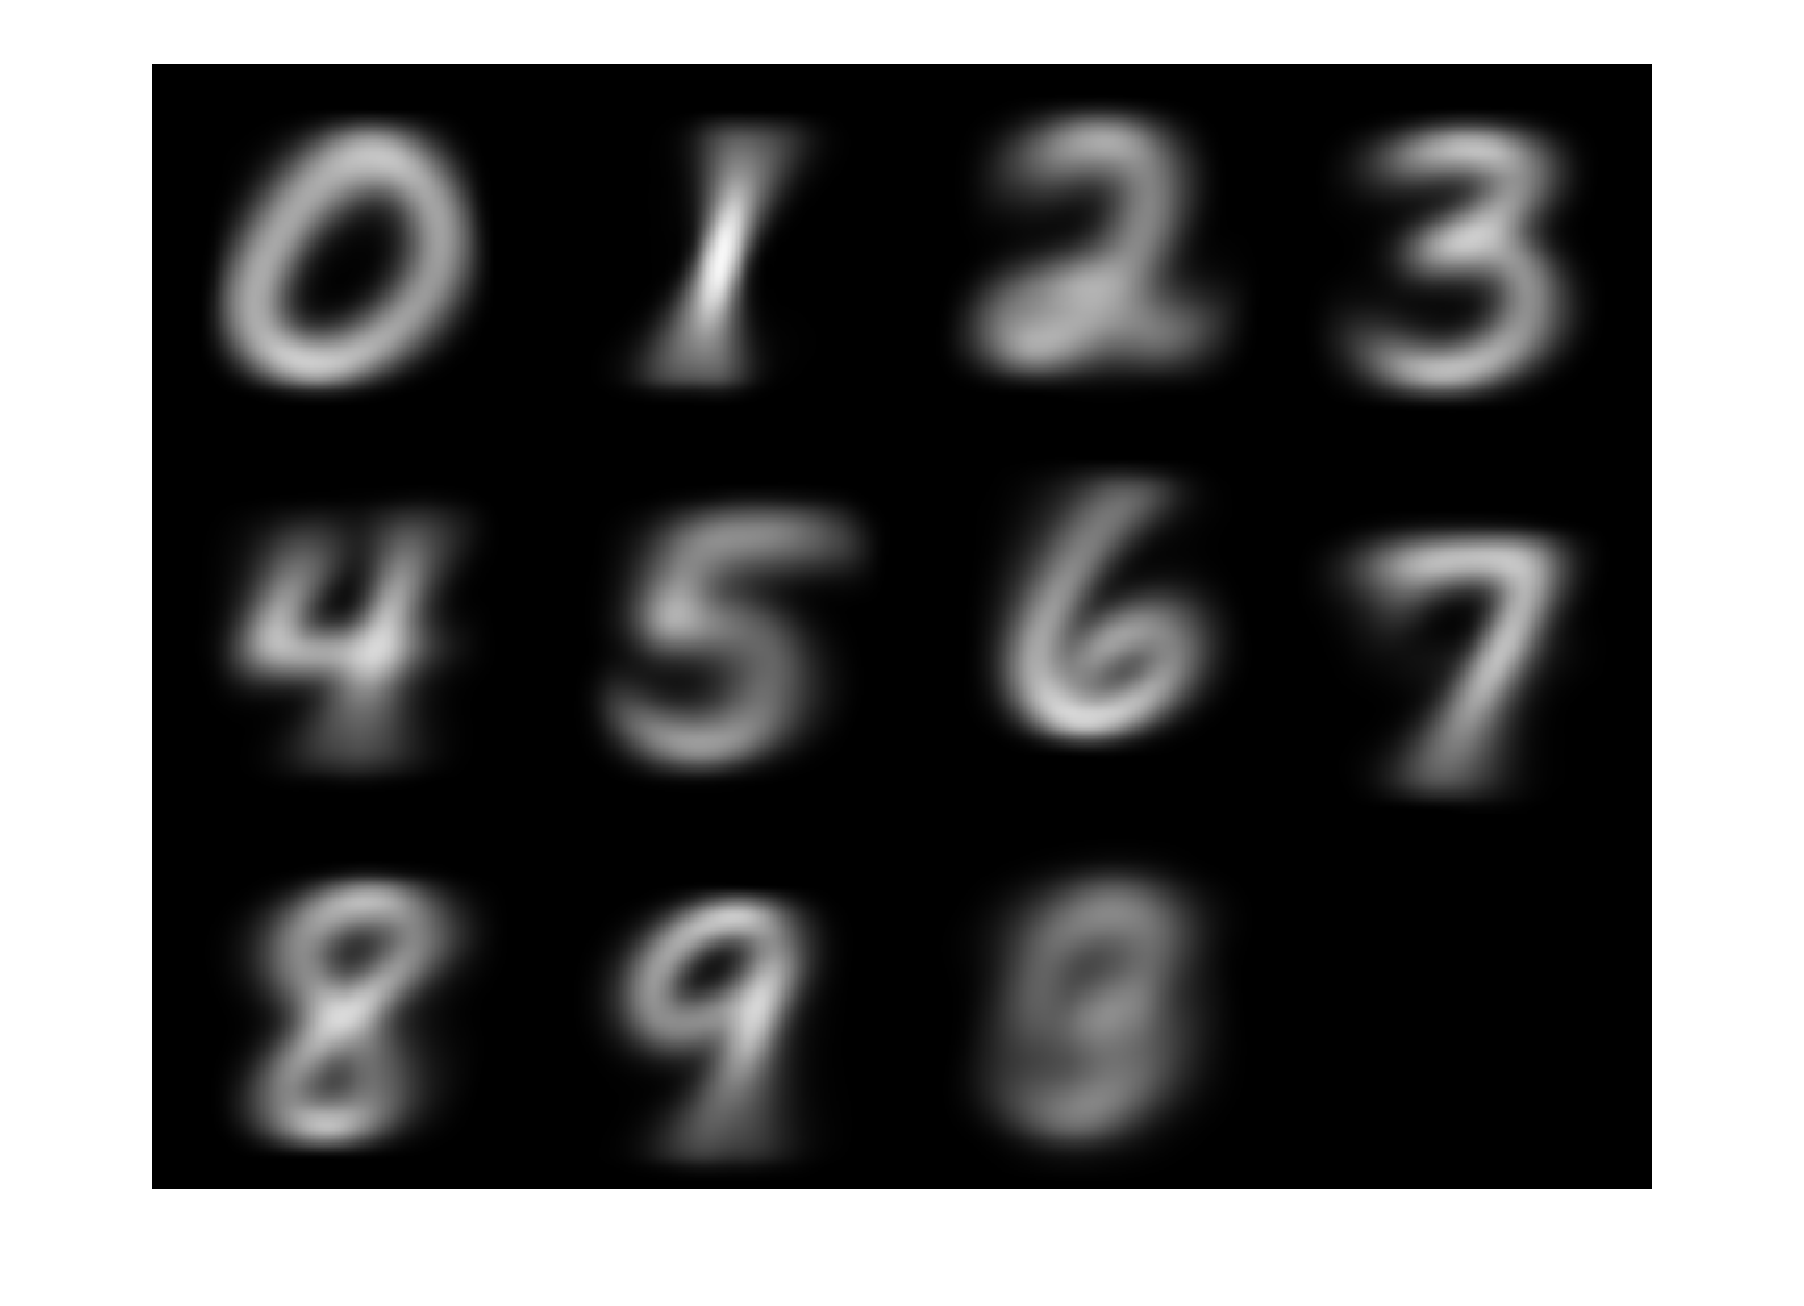
\includegraphics[width=150mm]{task1_2_imgs.eps}
 \caption{Task 1.2 - Montage of mean vectors}
\end{figure}
\begin{figure}
 \centering
	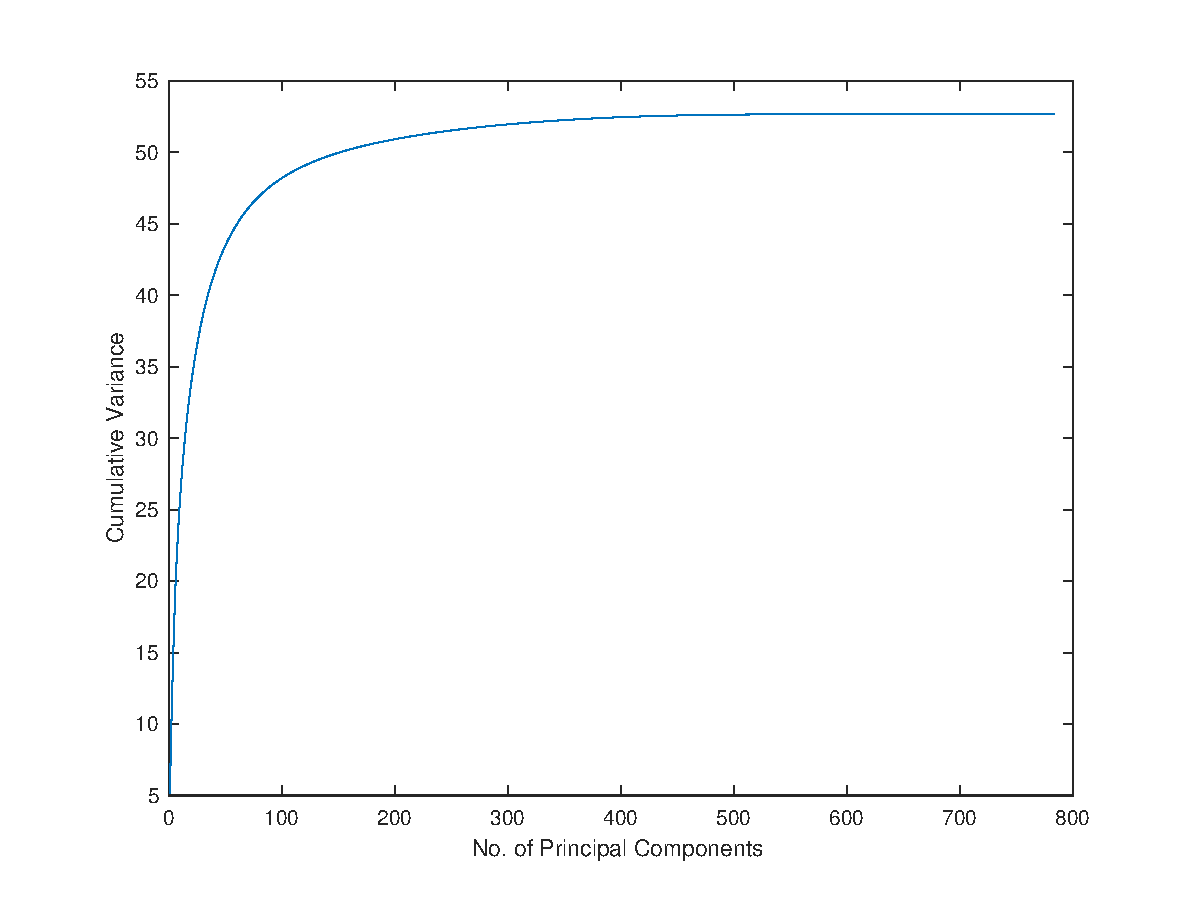
\includegraphics[width=150mm]{task1_3_graph.eps}
 \caption{Task 1.3 - Cumulative Variances}
\end{figure}
\begin{figure}
\centering
\begin{tabular}{l*{6}{c}r}
Variance      &      Components \\
\hline
70\% & 26   \\
80\%            & 44   \\
90\%           & 87   \\
95\%           & 154 \\
\end{tabular}
\end{figure}
\newpage
\begin{figure}
\centering
	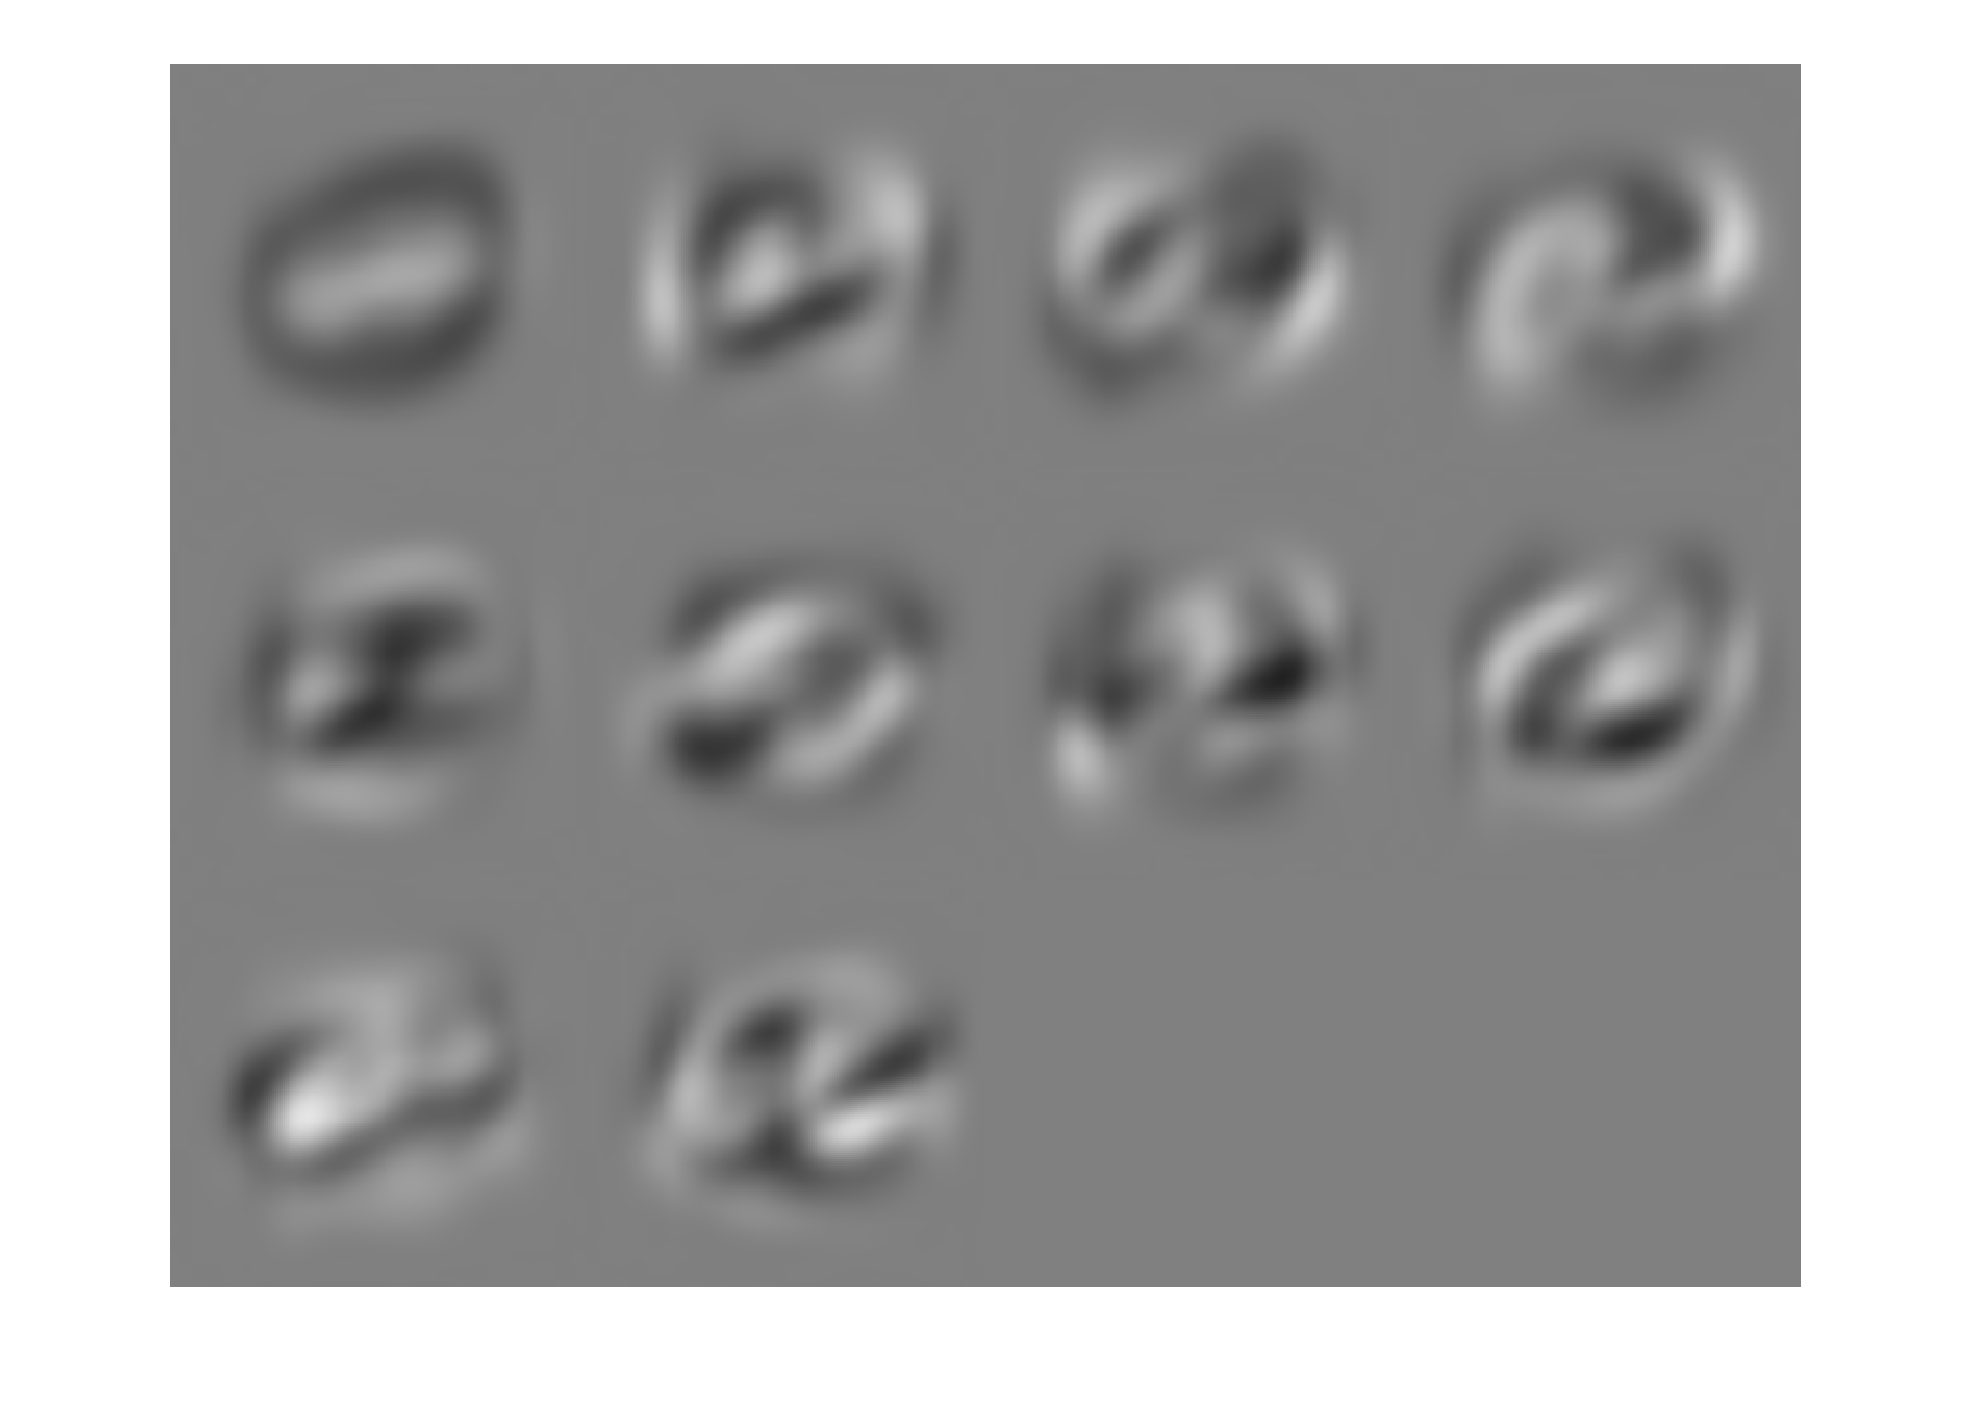
\includegraphics[width=170mm]{task1_4_imgs.eps}
	   \caption{Task 1.4 - First ten principal components}
\end{figure}
\end{document}